This section outlines how to collect IDE usage data using Eclipse's Usage Data
Collector (UDC).\footnote{\url{http://www.eclipse.org/epp/usagedata/}}
The UDC framework was originally build by the Eclipse Foundation, as a way to measure how the
community was using the Eclipse IDE.
While UDC was included in official Eclipse releases and data was collected from
hundreds of thousands of Eclipse users between 2008 and 2011, the project was eventually shut down,
and UDC was removed from official Eclipse releases.
However, the source code for UDC remains available and researchers can still use and deploy it.

\subsubsection{What Data is Collected}

The Eclipse Data Collector records the following types of Eclipse information:

\begin{itemize}

\item The runtime environment, such as the operating system and Java Virtual Machine.

\item Environment data, such as which bundles are loaded and when Eclipse
starts up and shuts down

\item Actions and commands that are executed, via menus, buttons, toolbars, and hotkeys.

\item Views, editors, and perspectives that are invoked.

\end{itemize}

\noindent
Let's look at an example of an event that UDC produces on a developer's machine:
\vspace{4mm}

\noindent
\begin{small}
\begin{tabular}{llllll}
\textbf{what}&\textbf{kind}&\textbf{bundleId}&\textbf{bundleVersion}&\textbf{description}&\textbf{time}\\
\hline
executed&command&org.eclipse.ui&3.7.0.v20110928-1505&org.eclipse.ui.edit.paste&1389111843130\\
\end{tabular}
\end{small}

\vspace{4mm}
\noindent
The first column tells us what kind of thing happened -- in this case, something was executed.
The second column tells us what was executed -- in this case, a command.
The third column tells us what bundle this event belonged to -- in this case, Eclipse's user interface bundle.
The fourth column gives us the version of the bundle.
The fifth tells us the name of the command that was executed -- in this case, paste.
The final column tells us when the command was executed, in Greenwich Mean Time -- in this case, January 7th, 2014 at 16:24:03 GMT.


\subsubsection{Limitations}

Apart from general limitations of collecting usage data (Section~\ref{sec:limitations}),
one significant limitation of UDC that we have found is that sometimes it has
unexpectedly incomplete data.
For example, in planning for a study involving when people ran their JUnit tests,
we found that UDC recorded an event when the ``Run \textgreater~Run As \textgreater~Run as JUnit Test'' menu item was selected,
but not when the ``Run As'' button was pressed on the toolbar.
We suspect that the reason has to do with how different user interface accordances
invoke the same functionality.
In general, when you are planning on running a study with UDC, be sure to know what
types of events you are looking for, and test them to make sure UDC captures those events.

\subsubsection{How to Use It}

\label{SecUDCHowToUseIt}

Collecting data for your own research is fairly straightforward with Eclipse UDC,
and we describe how to do so here.
We also include an accompanying screencast that shows the
basics.\footnote{\url{https://docs.google.com/file/d/0B7DV-T4_2mpKRWgwRnJnTWpvN0E/edit}}
%TODO move this screencast to youtube, once you're happy

\paragraph{Gathering Data Using the UDC Client.}

Let's talk about how data is collected on a developer's machine.
Since UDC was last included in the Eclipse Indigo SR2
release,\footnote{(\url{http://www.eclipse.org/downloads/packages/release/indigo/sr2}}
if you have the option of which Eclipse to use, we recommend downloading
that version.
By default, UDC starts collecting data when Eclipse is start up.
You can verify this by going to ``Windows \textgreater~Preferences'', then
select the ``Usage Data Collector'' item (Figure~\ref{fig:prefPage1}).
The \textit{Enable capture} option should be checked.

\begin{figure}
  \centering
  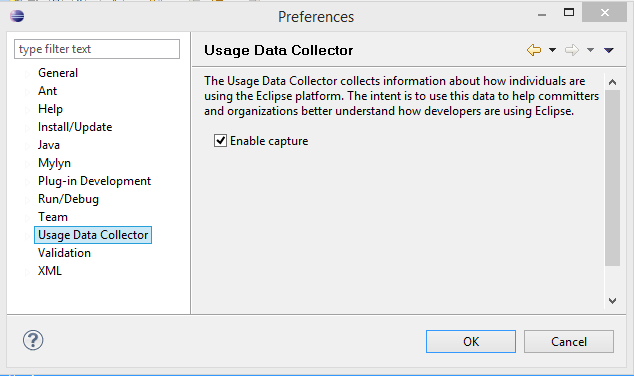
\includegraphics[scale=.58]{prefPage1}
  \caption{Eclipse Usage Data Collector preference page.}\label{fig:prefPage1}
\end{figure}

Before looking at the data, execute a few commands and open a few views
in Eclipse.
Then, on your file system, open the following path as a subdirectory
of your current workspace (Figure~\ref{fig:filesystem}):

\vspace{4mm}
\texttt{.metadata/.plugins/org.eclipse.epp.usagedata.recording}
\vspace{4mm}

\noindent
In that folder, depending on how many UDC events have been gathered,
a number of comma separated value (CSV) files will appear, where \texttt{upload0.csv} is the oldest
and \texttt{usagedata.csv} is the newest.
Open up \texttt{usagedata.csv} -- you should notice a large number and a variety of events.
Be sure to look specifically for events that you executed and views that you opened earlier.

\begin{figure}
  \centering
  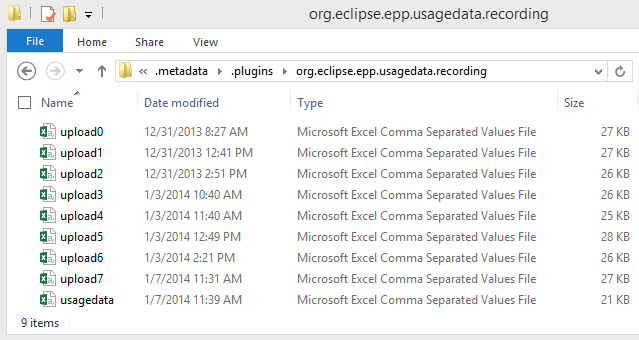
\includegraphics[scale=.58]{filesystem}
  \caption{UDC data files.}\label{fig:filesystem}
\end{figure}

Before doing a study, be aware that Eclipse will ask and periodically attempt to upload
data to the Eclipse foundation server.
You should \emph{not} allow it to do this, because each time data is uploaded, the underlying
CSV files are deleted.
Furthermore, because the UDC project is no longer officially supported, the official Eclipse
UDC server no longer accepts the data, so your usage data is, in effect, lost permanently.
Unfortunately, there is no easy way to tell the UDC client to permanently store
usage data.
An easy workaround is to increase the upload period to 90 days (Figure~\ref{fig:upload}),
which should be enough time to complete the experiment.
The long-term fix for this issue is to modify the source code, as we will explain
how to do shortly, to never upload data.

\begin{figure}
  \centering
  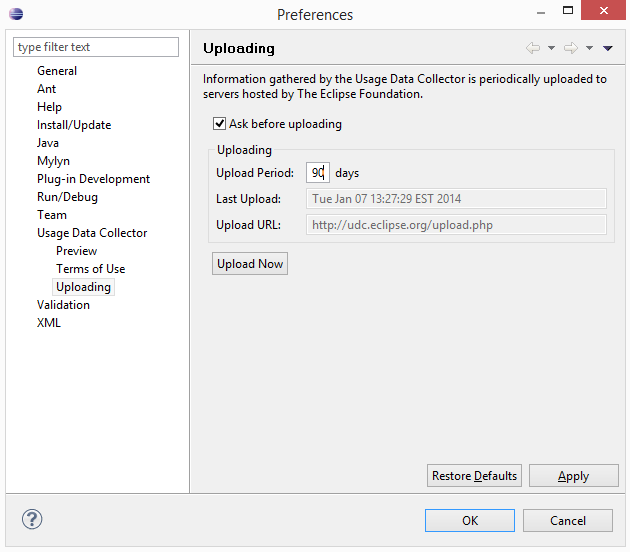
\includegraphics[scale=.58]{upload}
  \caption{Changing the UDC upload frequency.}\label{fig:upload}
\end{figure}

If you're doing a lab experiment, collecting data should be simply a matter of
copying and deleting the CSV files after each participant has done the experiment.
You can append the files together or put them in a database for analysis.

\paragraph{Modifying the UDC Client.}

You may wish to modify the UDC client yourself, perhaps to add a custom filter for events
or to disable data uploading.
Whatever the reason, making modifications to the client is fairly easy.

The first step is to check out the UDC source code into your Eclipse
workspace using git.\footnote{\url{http://git-scm.com/}}
Here we will again use Eclipse Indigo SR2, but we will specifically be using the
``Eclipse for RCP and RAP Developers'' download package because we will
modify Eclipse plugins.
Before importing the necessary plugins, we recommend switching to
the Indigo SR2 tag, to assure compatibility with
Eclipse.
To do so, clone the git repository\footnote{\url{http://git.eclipse.org/c/epp/org.eclipse.epp.usagedata.git/}}
locally, open up ``Tags'', right click on ``Indigo SR 2'',
then choose ``Checkout''.

To import the projects into Eclipse, right click on the repository, then click
``Import Projects,'' then ``Import Existing Projects.''
The three core projects to import are:

\begin{itemize}
\item org.eclipse.epp.usagedata.internal.gathering
\item org.eclipse.epp.usagedata.internal.recording
\item org.eclipse.epp.usagedata.internal.ui
\end{itemize}

Next, we recommend a quick smoke test to determine whether you
can actually make changes to the UDC client.
Open \texttt{UsageDataRecordingSettings.java}, then modify the value of \texttt{UPLOAD\_URL\_DEFAULT}
to \texttt{"my\_changed\_server"}.
Then, create a new debug configuration that is an Eclipse Application, and press
``Debug'' (Figure~\ref{fig:debugconfig}).
Finally, you can verify that your change worked by going to UDC's Uploading
preference page, noticing that the Upload URL is now ``my\_changed\_server''.

\begin{figure}
  \centering
  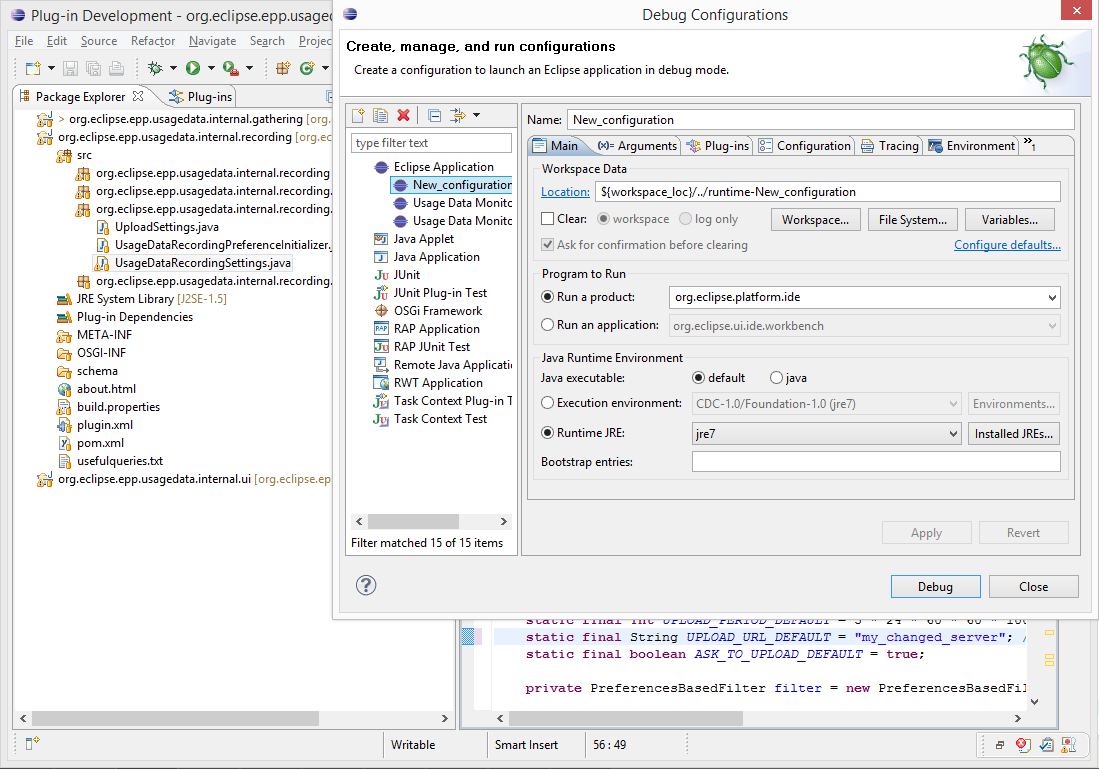
\includegraphics[scale=.58]{debugconfig}
  \caption{Debugging the UDC client.}\label{fig:debugconfig}
\end{figure}

From here, you can make any changes to the UDC client that you wish.
One thing you may want to do is upgrade UDC to work with more recent versions
of Eclipse.
The code is likely currently out of date
because it has not been maintained since the UDC project was shut down.
Another thing you may wish to do is deploy your new version of UDC via
an Eclipse update site to the developers you want to study.
There are many resources on the web for plugin deployment instructions,
such as Lars Vogel's tutorial on creating
plugins.\footnote{\url{http://www.vogella.com/tutorials/EclipsePlugIn/article.html#deployplugin_tutorial}}

\paragraph{Transmitting Data over the Internet.}

If you do not plan on doing a lab study where you can manually collect UDC usage
files, you will want to have the UDC client send the data to you directly.
As we mentioned, the best way to do this is probably by changing the default
server URL in the client source code.
An easy way to change the server when debugging is by adding the following Java
virtual machine arguments:

\vspace{4mm}
\texttt{-Dorg.eclipse.epp.usagedata.recording.upload-url=http://localhost:8080}
\vspace{4mm}

\noindent
However, simply changing the client to point at a new URL is insufficient,
because there actually has to be a working server at that URL, ready to
receive UDC data.
%%WBS: It is a bit confusing to talk about the PHP code as not working then talk about the server based on apache.  Why both?
While the source code of official Eclipse server was not officially made
available, Wayne Beaton from the Eclipse Foundation unofficially released
some of the PHP code from the Eclipse Foundation's server.
If you would like to download that code, you will find it in our git repository.
%TODO need to put this code into git
However, our PHP skills are very basic and we were not immediately able
to get the server working as expected, but we expect that anyone familiar with
debugging PHP should be able to.

\newpage

Creating your own server that receives UDC data is fairly straightforward.
Let's create a simple one using Apache's HttpComponents library,
the same library that UDC uses to upload data.
Specifically, we can create a server by simply extending Apache's tutorial
web server.\footnote{\url{http://hc.apache.org/httpcomponents-core-ga/httpcore/examples/org/apache/http/examples/ElementalHttpServer.java}}
First, we'll need a generic request handler to wait for HTTP connections:

\begin{lstlisting}
import java.io.IOException;
import org.apache.http.ConnectionClosedException;
import org.apache.http.HttpException;
import org.apache.http.HttpServerConnection;
import org.apache.http.protocol.BasicHttpContext;
import org.apache.http.protocol.HttpContext;
import org.apache.http.protocol.HttpService;

/**
 * Based on
 * http://hc.apache.org/httpcomponents-core-ga/httpcore/examples/org/apache
 * /http/examples/ElementalHttpServer.java
 */
class WorkerThread extends Thread {

	private final HttpService httpservice;
	private final HttpServerConnection conn;

	public WorkerThread(final HttpService httpservice, final HttpServerConnection conn) {
		super();
		this.httpservice = httpservice;
		this.conn = conn;
	}

	@Override
	public void run() {
		System.out.println("New connection thread");
		HttpContext context = new BasicHttpContext(null);
		try {
			while (!Thread.interrupted() && this.conn.isOpen()) {
				this.httpservice.handleRequest(this.conn, context);
			}
		} catch (ConnectionClosedException ex) {
			System.err.println("Client closed connection");
		} catch (IOException ex) {
			System.err.println("I/O error: " + ex.getMessage());
		} catch (HttpException ex) {
			System.err.println("Unrecoverable HTTP protocol violation: " + ex.getMessage());
		} finally {
			try {
				this.conn.shutdown();
			} catch (IOException ignore) {
			}
		}
	}
}
\end{lstlisting}

\newpage
\noindent
We'll also need a generic request listener:

\begin{lstlisting}
import java.io.IOException;
import java.io.InterruptedIOException;
import java.net.ServerSocket;
import java.net.Socket;

import org.apache.http.HttpConnectionFactory;
import org.apache.http.HttpServerConnection;
import org.apache.http.impl.DefaultBHttpServerConnection;
import org.apache.http.impl.DefaultBHttpServerConnectionFactory;
import org.apache.http.protocol.HttpService;

/**
 * Based on
 * http://hc.apache.org/httpcomponents-core-ga/httpcore/examples/org/apache
 * /http/examples/ElementalHttpServer.java
 */
class RequestListenerThread extends Thread {

	private final HttpConnectionFactory<DefaultBHttpServerConnection> connFactory;
	private final ServerSocket serversocket;
	private final HttpService httpService;

	public RequestListenerThread(final int port, final HttpService httpService)
			throws IOException {
		this.connFactory = DefaultBHttpServerConnectionFactory.INSTANCE;
		this.serversocket = new ServerSocket(port);
		this.httpService = httpService;
	}

	@Override
	public void run() {
		System.out.println("Listening on port " + this.serversocket.getLocalPort());
		while (!Thread.interrupted()) {
			try {
				// Set up HTTP connection
				Socket socket = this.serversocket.accept();
				System.out.println("Incoming connection from" + socket.getInetAddress());
				HttpServerConnection conn = this.connFactory.createConnection(socket);

				// Start worker thread
				Thread t = new WorkerThread(this.httpService, conn);
				t.setDaemon(true);
				t.start();
			} catch (InterruptedIOException ex) {
				break;
			} catch (IOException e) {
				System.err.println("I/O error initialising connection thread: " + e.getMessage());
				break;
			}
		}
	}
}
\end{lstlisting}

\newpage
\noindent
And finally, the guts of our server:

\begin{lstlisting}
import java.io.IOException;
import org.apache.http.HttpEntityEnclosingRequest;
import org.apache.http.HttpException;
import org.apache.http.HttpRequest;
import org.apache.http.HttpResponse;
import org.apache.http.protocol.HttpContext;
import org.apache.http.protocol.HttpProcessor;
import org.apache.http.protocol.HttpProcessorBuilder;
import org.apache.http.protocol.HttpRequestHandler;
import org.apache.http.protocol.HttpService;
import org.apache.http.protocol.ResponseConnControl;
import org.apache.http.protocol.ResponseContent;
import org.apache.http.protocol.ResponseDate;
import org.apache.http.protocol.ResponseServer;
import org.apache.http.protocol.UriHttpRequestHandlerMapper;
import org.apache.http.util.EntityUtils;

/**
 * Based on
 * http://hc.apache.org/httpcomponents-core-ga/httpcore/examples/org/apache
 * /http/examples/ElementalHttpServer.java
 */
public class BasicUDCServer {

		public static void main(String[] args) throws IOException {

		int port = 8080;

		HttpProcessor httpproc = HttpProcessorBuilder.create()
				.add(new ResponseDate()).add(new ResponseServer())
				.add(new ResponseContent()).add(new ResponseConnControl()).build();

		UriHttpRequestHandlerMapper reqistry = new UriHttpRequestHandlerMapper();
		reqistry.register("*", new HttpRequestHandler() {

			public void handle(HttpRequest request, HttpResponse response,
					HttpContext context) throws HttpException, IOException {

				HttpEntityEnclosingRequest entityRequest = (HttpEntityEnclosingRequest) request;

				String userID = request.getHeaders("USERID")[0].getValue();
				String workspaceID = request.getHeaders("WORKSPACEID")[0].getValue();
				long time = Long.parseLong(request.getHeaders("TIME")[0].getValue());

				System.out.println(userID + "," + workspaceID + "," + time);
				System.out.println(EntityUtils.toString(entityRequest.getEntity()));
			}
		});

		HttpService httpService = new HttpService(httpproc, reqistry);

		Thread t = new RequestListenerThread(port, httpService);
		t.setDaemon(false);
		t.start();
	}
}
\end{lstlisting}

\noindent
When this server is run and it receives a UDC upload,
it will print a UserId, WorkspaceId, and time the upload was sent.
UserIds are randomly generated on the client side and stored in a file in
the user's home directory.
As long as that file remains intact, future uploads from that user will
contain that UserId.
WorkspaceIds are identifiers contained in each workspace, and can be
used to uniquely (but anonymously) identify which
workspace a set of data is uploaded from.
Thus, there is normally only one UserId per computer, but there can
be multiple WorkspaceIds per computer.

This code can be modified to fit your needs.
We have provided a github repository where you can checkout
and change this code as you see fit.
%TODO provide code on server
%TODO: Please craft a short conclusion paragraph (3 sentences max) to the UDC section.  Think about final words of advice to the researcher.  Thanks WBS